%%
%% This is file `sample-sigconf.tex',
%% generated with the docstrip utility.
%%
%% The original source files were:
%%
%% samples.dtx  (with options: `all,proceedings,bibtex,sigconf')
%%
%% IMPORTANT NOTICE:
%%
%% For the copyright see the source file.
%%
%% Any modified versions of this file must be renamed
%% with new filenames distinct from sample-sigconf.tex.
%%
%% For distribution of the original source see the terms
%% for copying and modification in the file samples.dtx.
%%
%% This generated file may be distributed as long as the
%% original source files, as listed above, are part of the
%% same distribution. (The sources need not necessarily be
%% in the same archive or directory.)
%%
%%
%% Commands for TeXCount
%TC:macro \cite [option:text,text]
%TC:macro \citep [option:text,text]
%TC:macro \citet [option:text,text]
%TC:envir table 0 1
%TC:envir table* 0 1
%TC:envir tabular [ignore] word
%TC:envir displaymath 0 word
%TC:envir math 0 word
%TC:envir comment 0 0
%%
%%
%% The first command in your LaTeX source must be the \documentclass
%% command.
%%
%% For submission and review of your manuscript please change the
%% command to \documentclass[manuscript, screen, review]{acmart}.
%%
%% When submitting camera ready or to TAPS, please change the command
%% to \documentclass[sigconf]{acmart} or whichever template is required
%% for your publication.
%%
%%
\documentclass[bibtex, sigconf, hyperref={colorlinks=true,linkcolor=blue,urlcolor=blue}]{acmart}

%%
%% \BibTeX command to typeset BibTeX logo in the docs
\AtBeginDocument{%
  \providecommand\BibTeX{{%
    Bib\TeX}}}

%% Rights management information.  This information is sent to you
%% when you complete the rights form.  These commands have SAMPLE
%% values in them; it is your responsibility as an author to replace
%% the commands and values with those provided to you when you
%% complete the rights form.

% Is this necessary for us?
\setcopyright{acmlicensed}
\copyrightyear{2024}
\acmYear{2024}
\acmDOI{XXXXXXX.XXXXXXX}

%% These commands are for a PROCEEDINGS abstract or paper.
% \acmConference[Conference acronym 'XX]{Make sure to enter the correct
%   conference title from your rights confirmation emai}{June 03--05,
%   2018}{Woodstock, NY}
%%
%%  Uncomment \acmBooktitle if the title of the proceedings is different
%%  from ``Proceedings of ...''!
%%
%%\acmBooktitle{Woodstock '18: ACM Symposium on Neural Gaze Detection,
%%  June 03--05, 2018, Woodstock, NY}
% \acmISBN{978-1-4503-XXXX-X/18/06}


%%
%% Submission ID.
%% Use this when submitting an article to a sponsored event. You'll
%% receive a unique submission ID from the organizers
%% of the event, and this ID should be used as the parameter to this command.
%%\acmSubmissionID{123-A56-BU3}

%%
%% For managing citations, it is recommended to use bibliography
%% files in BibTeX format.
%%
%% You can then either use BibTeX with the ACM-Reference-Format style,
%% or BibLaTeX with the acmnumeric or acmauthoryear sytles, that include
%% support for advanced citation of software artefact from the
%% biblatex-software package, also separately available on CTAN.
%%
%% Look at the sample-*-biblatex.tex files for templates showcasing
%% the biblatex styles.
%%

%%
%% The majority of ACM publications use numbered citations and
%% references.  The command \citestyle{authoryear} switches to the
%% "author year" style.
%%
%% If you are preparing content for an event
%% sponsored by ACM SIGGRAPH, you must use the "author year" style of
%% citations and references.
%% Uncommenting
%% the next command will enable that style.
%%\citestyle{acmauthoryear}


%%
%% end of the preamble, start of the body of the document source.
\begin{document}

%%
%% The "title" command has an optional parameter,
%% allowing the author to define a "short title" to be used in page headers.
\title{Predictors of NFL Tackles}

%%
%% The "author" command and its associated commands are used to define
%% the authors and their affiliations.
%% Of note is the shared affiliation of the first two authors, and the
%% "authornote" and "authornotemark" commands
%% used to denote shared contribution to the research.
\author{Isaac Kou (4502)}
\email{Isaac.Kou@colorado.edu}
\affiliation{%
  \institution{University of Colorado Boulder}
  \city{Boulder}
  \state{Colorado}
  \country{USA}
}

\author{Sean Shi (4502)}
\email{Sean.Shi@colorado.edu}
\affiliation{%
  \institution{University of Colorado Boulder}
  \city{Boulder}
  \state{Colorado}
  \country{USA}
}

\author{Timur Tripp (5502)}
\email{Timur.Tripp@colorado.edu}
\affiliation{%
  \institution{University of Colorado Boulder}
  \city{Boulder}
  \state{Colorado}
  \country{USA}
}

% \author{Grace Williams (5502)}
% \email{grwi3115@colorado.edu}
% \affiliation{%
%   \institution{University of Colorado Boulder}
%   \city{Boulder}
%   \state{Colorado}
%   \country{USA}
% }

% \authornote{Both authors contributed equally to this research.}
% \orcid{1234-5678-9012}
% \author{G.K.M. Tobin}
% \authornotemark[1]
% \affiliation{%
%   \institution{Institute for Clarity in Documentation}
%   \city{Dublin}
%   \state{Ohio}
%   \country{USA}
% }

%%
%% By default, the full list of authors will be used in the page
%% headers. Often, this list is too long, and will overlap
%% other information printed in the page headers. This command allows
%% the author to define a more concise list
%% of authors' names for this purpose.
\renewcommand{\shortauthors}{Kou et al.}

%%
%% The abstract is a short summary of the work to be presented in the
%% article.

\begin{abstract}
This paper analyzes the 2024 National Football League (NFL) Big Data Bowl dataset
which contains data from the 2022 season of the NFL.
We show that the height, weight, and position of the player in the game can
accurately predict whether or not the player made a tackle during that play.
Additionally, strategies such as the formation used by defense and offense
and the length of passes can increase or decrease the distance before tackle of
a carrier or the likelihood of a tackle succeeding.
\end{abstract}

%%
%% The code below is generated by the tool at http://dl.acm.org/ccs.cfm.
%% Please copy and paste the code instead of the example below.
%%

%%
%% Keywords. The author(s) should pick words that accurately describe
%% the work being presented. Separate the keywords with commas.
\keywords{Football, NFL, Data Mining, Tackles}

%% A "teaser" image appears between the author and affiliation
%% information and the body of the document, and typically spans the
%% page.

\begin{teaserfigure}
% Random image of tackling I pulled from the internet, feel free to replace
  % \caption{Seattle Mariners at Spring Training, 2010.}
  % \Description{Enjoying the baseball game from the third-base
  % seats. Ichiro Suzuki preparing to bat.}
  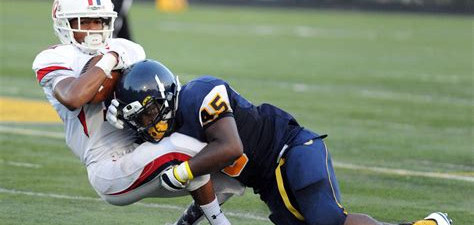
\includegraphics[width=\textwidth]{./th-4169371817}
  \label{fig:teaser}
\end{teaserfigure}

\received{15 December 2024}
% \received[revised]{12 March 2009}
% \received[accepted]{5 June 2009}

%%
%% This command processes the author and affiliation and title
%% information and builds the first part of the formatted document.
\maketitle

\section{Introduction}

Every year, the Nation Football League (NFL) hosts the NFL Big Data Bowl, an annual
sports data analytics competition in which teams analyze specific datasets
provided by Next Gen Stats in order to encourage data-backed improvements to the
NFL. The data, which aligns with the competition's yearly theme, is

\begin{quote}
\textit{``the capture of real time location data, speed and acceleration for
every player, every play on every inch of the field. Sensors throughout the
stadium track tags placed on players' shoulder pads, charting individual
movements within inches."}
\cite{nextgenstats}
% \raggedleft{[Next Gen Stats, 2024 \url{https://nextgenstats.nfl.com/glossary}]}
\end{quote}

Specifically, the 2024 Big Data Bowl focuses on the theme of tackling in order
to encourage the creation of metrics quantifying things like tackle probability,
play impacts, expected points, and injury.

Tackling is imperative to the sport of American football, as the defending
team's main goal is to tackle the opposing player with the football as soon as
possible in order to help prevent the team from scoring. As such, the dataset
used to analyze tackling includes categories on game data, play data, player
data, tackles data, and tracking data. The goal of this project is to utilize
such metrics in order to find correlations between known information such as
weight, height, and time during a game and the outcome of plays (whether or not
the tackle was completed, whether the tackle was successful in terms of
gameplay, etc.).

\section{Existing Work}

A significant number of previous academic studies exist on the topic of tackling
in American football. This section discusses three examples of those studies,
one hobbyist analysis, and the foundation they lay for our proposed work.

The paper
\href{https://link.springer.com/article/10.1007/s10439-020-02625-7}{“Validating
Tackle Mechanics in American Football: Improving Safety and
Performance”}\cite{validatingtackles} (Maerlender et al.) discusses the
development of a program to reduce the risk of serious injury from tackling,
specifically by identifying head-contact likelihoods and therefore alternative
techniques to reduce such contact. Secondary research related to the impact of
tackles on player performance was also conducted, finding a reduction in their
number of yards run post-contact.

Similarly,
\href{https://www.jstage.jst.go.jp/article/ijshs/16/0/16_201804/_article/-char/ja/}
{“Effectiveness of the Heads Up Tackling (HUT) Program on Tackling Safety and
Performance in American Football”}\cite{effectiveness} (Matsuo et al.) also
identifies a program to promote tackle safety, though this study focuses on an
existing program and its observed impacts. Results indicated that implementation
of the studied HUT Program reduced rate and severity of player injury, with no
detriment, or, in some cases, even benefit, to player performance.

Lastly,
\href{https://bmjopensem.bmj.com/content/6/1/e000638.abstract}{“Quantitative and
qualitative analysis of head and body impacts in American 7v7 non-tackle
football”}\cite{quantitative} (Jadischke et al.) used video analysis to
investigate the rate of head contact in the alternative non-tackle play style of
American football. In a similar vein to the above studies, this research found
that non-tackle football was associated with lower rates of head contact and
therefore potentially lower rates of injury, though further research is needed.

Outside of academia, many football fans conduct hobbyist analyses of their own,
often concerning points, player performance, game trends, and so on. An example
of this is the article
\href{https://medium.com/@ezra.ford/tackling-metrics-with-big-data-0812b5ab65f0}{“Tackling
Metrics with Big Data”} by Ezra Ford on Medium. In addition to being a subject
of interest in and of themselves, these have applications in related
sub-hobbies, such as sports betting and fantasy football, and can help fans
maximize their success in those activities.

As shown, the existing work on tackles in American football often concerns the
implications of tackling, instead of the ability to predict and understand
when/where/how tackles happen.  Thus, our work intends to investigate these
trends instead.

\section{Methodology}

In this project, we seek to find the effects of different attributes on the
success rate and time of tackles and subsequently, how tackles effects the
outcome of a game.  To this end, we will be employing a variety of statistical
techniques covered in both CSCI4502/5502 and from other classes.

\subsection{Datasets}

To analyze the effect of various traits of player, matches, and other factors on
the timing and a success rate of tackle, we will primarily be using data from
the Kaggle NFL Big Data Bowl \cite{nflkaggle}
% \footnote{\url{https://www.kaggle.com/competitions/nfl-big-data-bowl-2024/data}}
specifically the files ``\verb|tackles.csv|'', ``\verb|games.csv|'',
``\verb|plays.csv|'' which contain data on the play, players, success, teams,
etc. involved in a tackle.  We will also be examining data from 9 weeks of
tracking data (``\verb|tracking_week_[1-9].csv|'') to determine the effects of
factors such as position on the field or movement at the time of a tackle.

\subsection{Exploratory analysis}

% TODO: Revise these two paragraphs to fit work already done:

Our primary goal for this project was to find correlations between previously
known information such as weight, height, and time during a game and the tackles
performed (location, likelihood of success and number of tackles). To this end,
we aimed to find correlations between factors such as height and
weight of player, and frequency and likelihood of success of tackles, as well as
frequency analysis for examining which teams/players tend to engage in tackles.
Analysis methods included both the na\"ive Bayes and decision tree classifiers.

Expanding beyond this, we also explored how strong of a correlation exists
between defensive players making or missing tackles and their team winning games.
We used data on the number of tackles performed during a game to see the effect on
the game's outcome. This was intended to provide insight on how tackles can affect the
course of the game.

Finally, we used compiled this information to determine potential strategies and implications
on real-world applications, including the selection of offensive strategies and the use of
certain formations.

\subsection{Grouping tackles}

When performing a tackle, the physical attributes of the players involved such
as their relative speed, direction, location, etc. may have an effect on how
tackles are performed and whether they are sucessful. By filtering tracking
data from ``\verb|tracking_week_[1-9].csv|'' on tackle events, we are able to
determine each player's movement at the moment of a tackle. Since this data is
largely numerical and are likely not independent, we have used cluster analysis
using a k-means algorithm to determine any patterns in the dataset.

Using the Elbow Method, we choose 5 clusters for this dataset and applied the
k-means methods to a number of combinations of attributes. By joining this
dataset with the plays dataset, we were also able to determine which plays are
more likely to have tackles and the relative motion of players with respect to
each other at the time of tackle.

\subsection{Offensive strategies}

NFL offenses are always looking for ways to stay ahead of defenses. Putting
ourselves in the shoes of an NFL offensive coordinator, we formulated three
potential offensive strategies to investigate.

\subsubsection{Optimizing the weight of running backs}

Many play designs involve the quarterback handing the ball off to a player
designated as the running back (RB), who attempts to run forward for as many
yards as possible before being tackled or forced out of bounds by the defense.

For this offensive strategy, we will check if optimizing the weight of a running
back is associated with a more favorable outcome for an increase in missed
tackles, and if playing heavier running backs is associated with a positive
impact on tackle performance.

\subsubsection{Increasing passing yards}

For a receiver, making catches is important, but just making the catch isn't all
that matters. Yards after catch, the distance a receiver travels after making a
catch but before a tackle, being forced out of bounds, or scoring, is also an
important metric. Higher yards after catch will result in more yards gained
during passing plays.

To increase yards after catch, offenses may need to make longer passes down the
field to areas where there are fewer defenders nearby to make the tackle. For
this offensive strategy, we analyze whether longer passes resulting in more yards
after catch is supported by the dataset.

Note that this analysis will only include plays where a pass was made which
requires filtering out observations without a value for \texttt{passLength}.

\subsubsection{Choosing specific offensive formation types}

An offensive coach must decide on a formation to use depending on what the play
is trying to achieve, e.g. short run or long pass. The game permits several
different formation types, with different formations placing players at
different locations behind the line of scrimmage, or the line which separates
offense and defense at the start of a play and marks the distance remaining for
a first down.

A formation also directs the movement of players after a play begins, based on
their positions in the game. For example, a wide receiver may be directed to run
down the field to provide a target for a pass. Defenses are allowed to respond
to offensive formations based on how the offensive players line up, but may not
always know the offense's full intentions.

For this offensive strategy, we will analyze offensive formations to see if any
formation types are associated with more favorable outcomes for offenses seeking
to increase the amount of plays with missed tackles. We will also determine how
offensive formation preferences change based on variables such as down and
distance.

\subsection{Tackles as a predictor of victory}

“The best offense is a good defense” and “defense wins championships” are
popular sayings, but is it really true? We will explore how strong of an
association exists between defensive players making or missing tackles and
their team winning games, and whether tackles can be used to predict game
outcomes.

\section{Evaluation}

\subsection{Exploratory analysis}

By analyzing the frequency of \verb|yardsToGo|, we were able to determine that
the vast majority of plays started at 10 yards to go. This is likely because
10 yards is the starting point for each round. We also see more observations
less than 10 yards to go than greater meaning moving forward is much more likely
than backwards. The slight increase observed at 15 or 20 yards to go is likely
due to penalties as -5 or -10 yards are common penalties.

\begin{figure}[h]
  \centering
  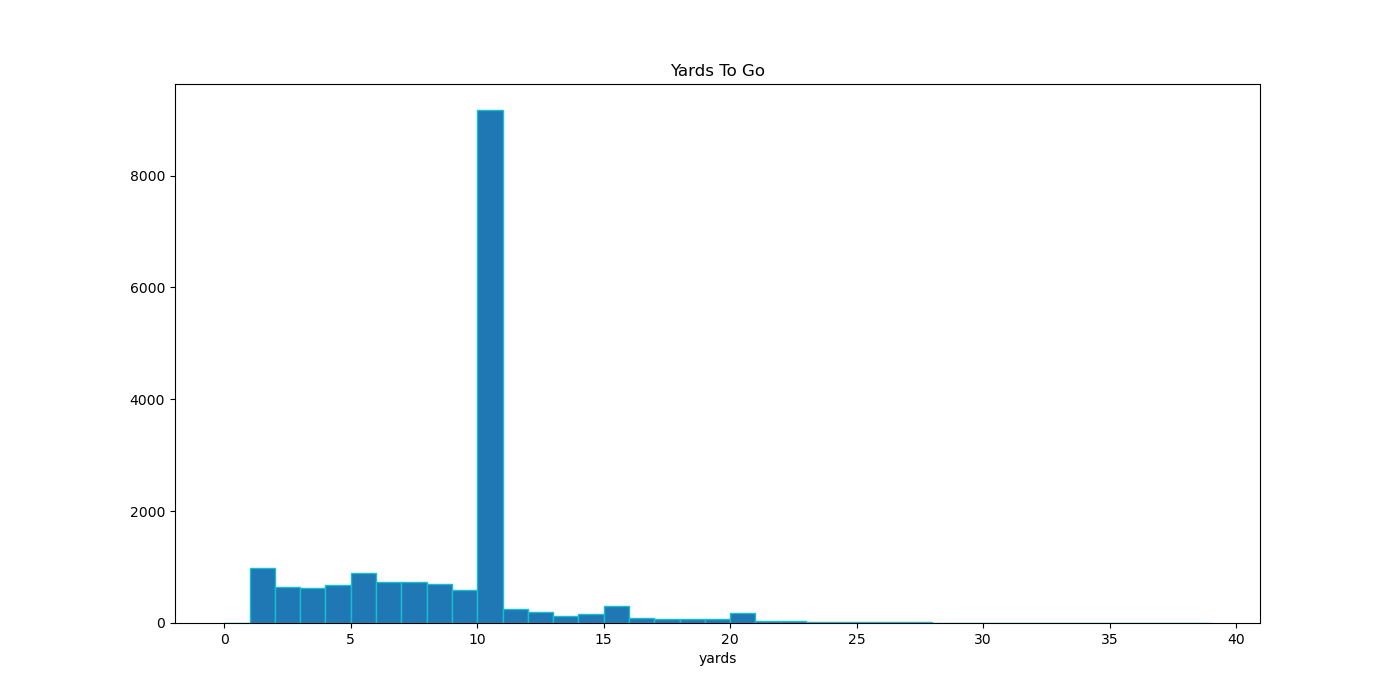
\includegraphics[width=\linewidth]{../src/yards.png}
  \caption{yards to go}
  \Description{A histogram of yards to go, has a peak at 10, more observations
  less than 10 than greater, and smaller peaks at 5, 10, -5, -10}
\end{figure}

This also shows that most tackles occur fairly close to the starting line of the play.

\subsection{Classifier Predictions of Tackle Success}

To determine if certain factors about the ball-carrying player (the player being tackled)
made a tackle more likely to succeed, we attempted to use both a na\"ive Bayesian
classifier and a decision tree classifier to predict the likelihood of a tackle succeeding
based on the following attributes:

\begin{itemize}
\item Weight: The player's height, in feet and inches, sorted into 3 categories: ($< 5'10'',
5'10''-6'2'', > 6'3''$, which were codenamed as "Short", "Average", and "Tall")
\item Height: The player's weight, in pounds, sorted into 3 categories (`Under 200', `200 -
250', `Over 250')
\item Position: The player's position on the team (FB, QB, RB, TE, WR)
\end{itemize}

Two different classifiers were chosen in order to compare the results. Meanwhile,
the attributes listed above were chosen because they were intrinsic to the player
and likely meaningful to the effect of the tackle, or involved with their role on the field
(reflecting possible influences such as positioning, play style, etc. and thus
meaningful to the game), and thus could inform decisions about how to be more successful
with future tackles.

We used $67\%$ of the data for training the Bayesian and decision tree models, and the rest for
testing each model's effectiveness in predicting success. Both resulting models were able to
predict whether or not a tackle succeeded with accuracy of $88.6\%$ and F1-score
of $0.9397763996855621$. This shows that the factors chosen were, at least at face value, effective in
predicting the likelihood of a tackle succeeding.

\begin{figure}[h]
  \centering
  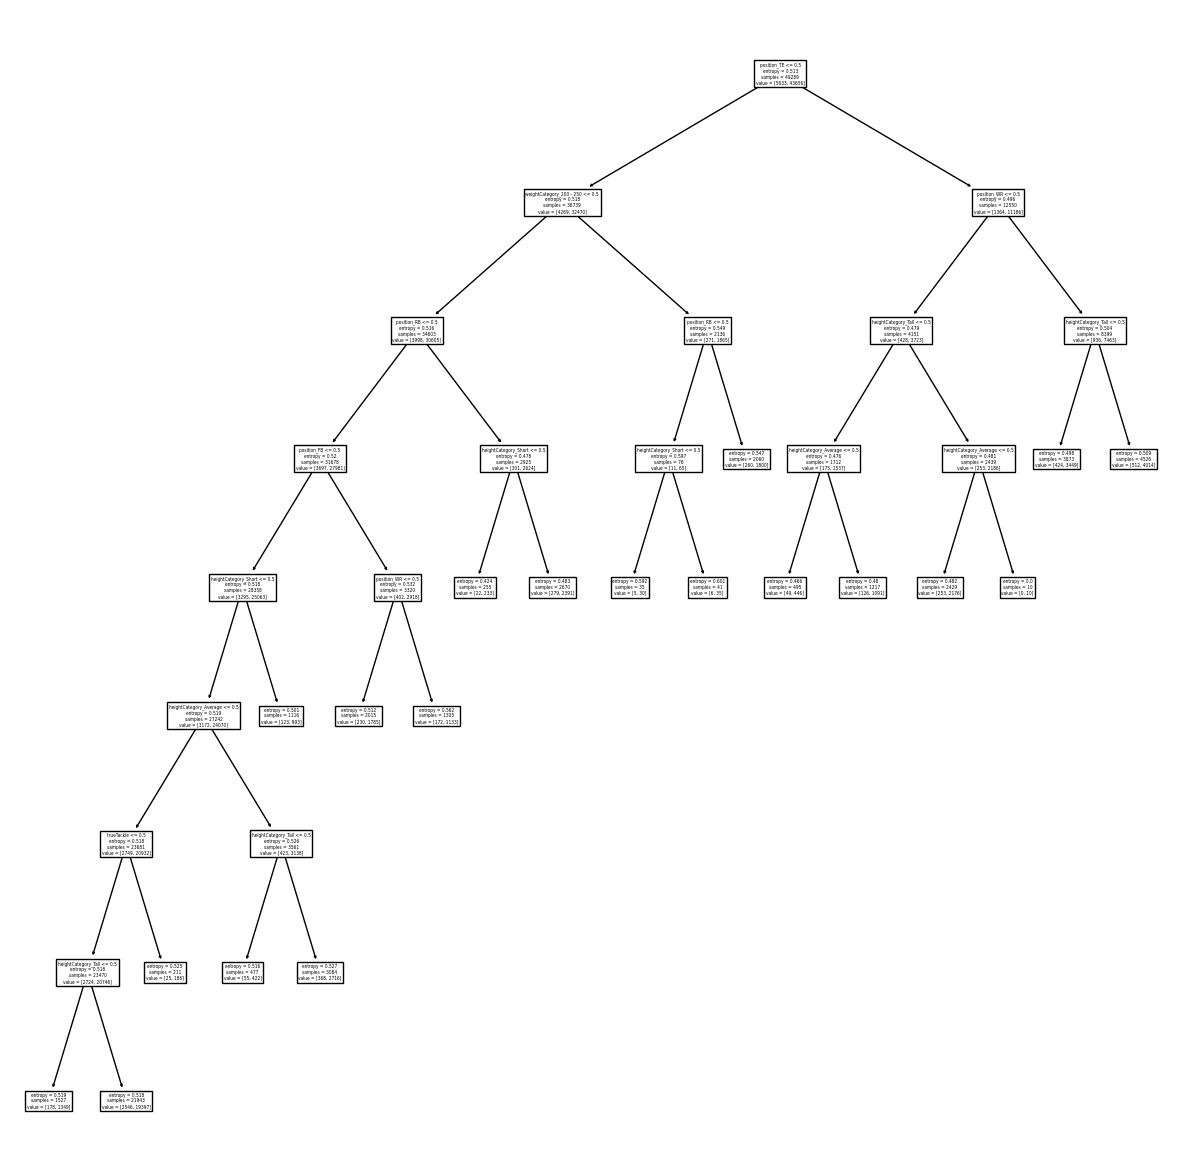
\includegraphics[width=\linewidth]
  {decision_tree.png}
  \caption{The resulting decision tree for tackle likelihood prediction.}
\end{figure}

However, it is worth noting that the dataset of tackles provided by the NFL had relatively few records
of "missed" tackles in comparison to "made" or "successful" tackles. This likely affected the accuracy
of the classifiers and made them seem more predictive than they are.

When the dataset was adjusted using SMOTE (Synthetic Minority Oversampling Technique), the
Bayesian model had an accuracy of $50.9\%$ and an F1-score of $0.5096858777515016$, while the
decision tree had an accuracy of $50.4\%$ and an F1-score of $0.6700675539890862$. This supports
the idea that the accuracy of the classifiers is inflated by the proportion of made to missed tackles,
and once balanced, their predictive abilities are no longer as strong.

\subsection{Grouping Tackles}

Using the $x$ and $y$ attributes of the tracking dataset which correspond to the
position of the football in yards at the time of the tackle, we attempted to
determine if there any patterns in position at the time of tackle.
We were unable to find significant clusters of positions where tackles
occurred. As shown in the figure below, the locations of tackles do not appear
to be in any statistically significant clusters. Notably, tackles tended to
occur much more frequently close to the center of the field in both the $x$ and
$y$ axes. One explanation for this is that players may be forced out of bounds
rather than tackled, which also ends the play.

\begin{figure}[h]
  \centering
  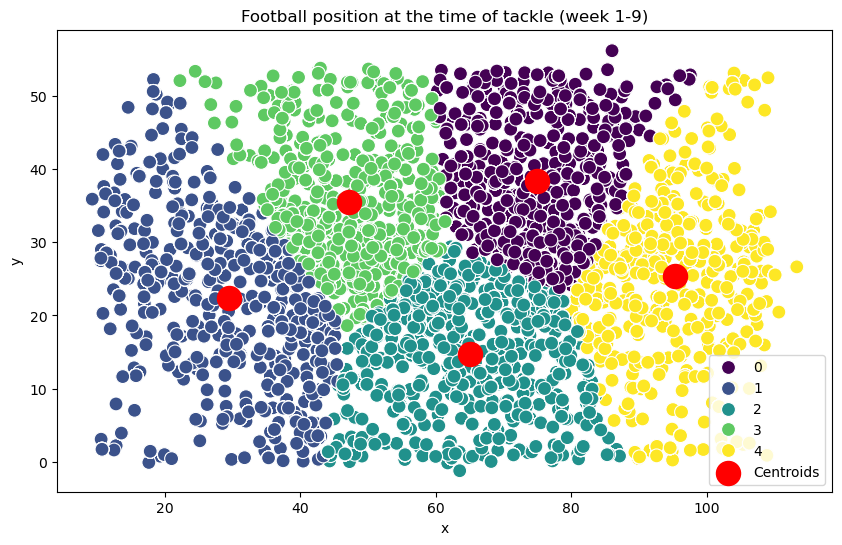
\includegraphics[width=\linewidth]{k-means}
  \caption{k-means analysis of football position}
  \Description{A plot of the x and y coordinates of tackles}
\end{figure}

By using speed and acceleration of the football which acts as a proxy for the
speed and acceleration of a player as they are being tackled, we are able to see
that most tackles are clustered at fairly low speeds and accelerations. A second
much smaller cluster of tackles also happen at low speeds but high accelerations.
One explanation for this is that most players are seeking to avoid injury, so
will not try to go faster if they are already likely to be tackled.

\begin{figure}[h]
  \centering
  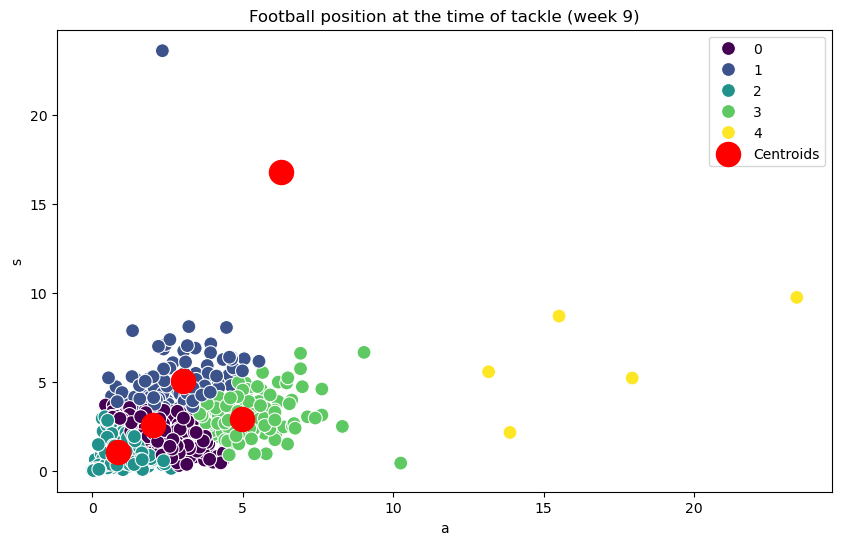
\includegraphics[width=\linewidth]{speed-accel}
  \caption{speed and acceleration at time of tackle}
\end{figure}

Additionally, by comparing the speed and direction of the ``tackler'' and the
ball carrier, we can see that in most cases, the 2 are traveling in the same
direction. However, the speed of the ball carrier tends to be higher than that
of the defender likely because they must respond to what the ball carrier is
doing and the ball carrier must outrun multiple defenders.
\begin{figure}[h]
  \centering
  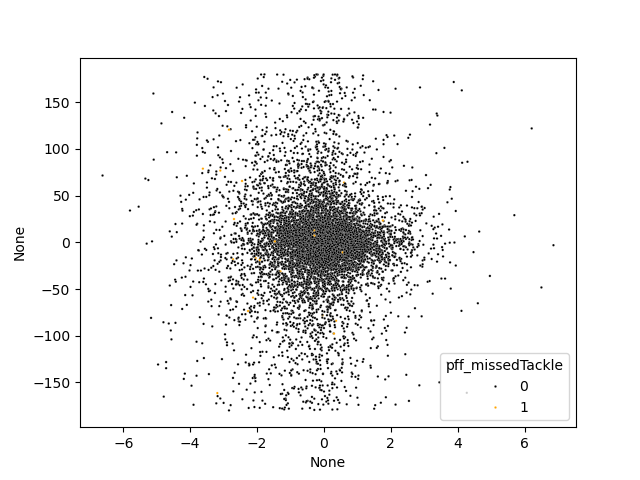
\includegraphics[width=\linewidth]{speed}
  \caption{difference in speed and direction between defender and ball carrier}
\end{figure}

\subsection{Comparing prediction models}

% TODO: Add results (Isaac & Tim)

When comparing the predictive models of tackle likelihood based on player
attributes, the differences between the na\"ive Bayes and decision tree
classifiers was very small. They had identical accuracy and F1-scores under the
original dataset, and very similar ones under the adjusted SMOTE dataset.
Thus, in terms of predictive power, neither is necessarily better than the
other. However, the decision tree offers a more easily interpretable visual
representation, while the Bayes model is more flexible in terms of programming
and individual predictions, so each has their own strengths and weaknesses in
practical use.

\subsection{Offensive strategies}

\subsubsection{Optimizing the Weight of Running Backs}

Running backs aren't significantly heavier than other offensive players. The
heaviest players play at the key blocker positions of center (C), offensive
guard (G), and offensive tackle (T), where the goal is to block defensive
players from entering the offensive backfield and running long distances is
rare. Players playing quarterback (QB), wide receiver (WR), and tight end (TE)
don't need to be as heavy to do their jobs effectively. Players playing at wide
receiver (WR) come in at the lightest weight, which makes sense for a player
needing to be agile enough to make mid-air catches.

\begin{figure}[h]
  \centering
  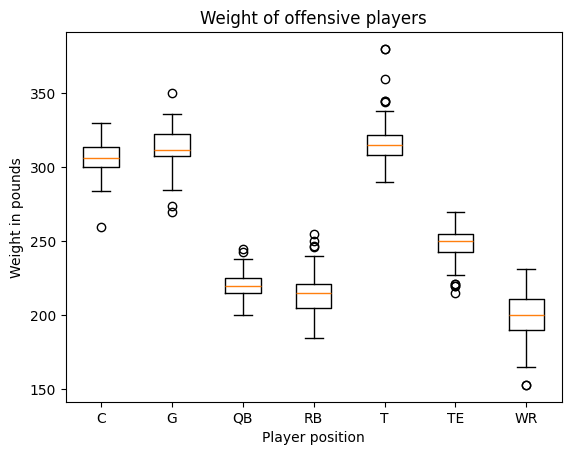
\includegraphics[width=\linewidth]{weight-of-offensive-players.png}
  \caption{Weight of offensive players, grouped by position}
\end{figure}

For the rest of this analysis, we focused on played running backs and removed
those who weren't involved in at least one play. The weight of played running
backs is roughly normally distributed, with a mean of 213.82 pounds and standard
deviation of 12.75 pounds. This was confirmed using a quartile-quartile (QQ)
probability plot, which also revealed some outliers at the tails.

\begin{figure}[h]
  \centering
  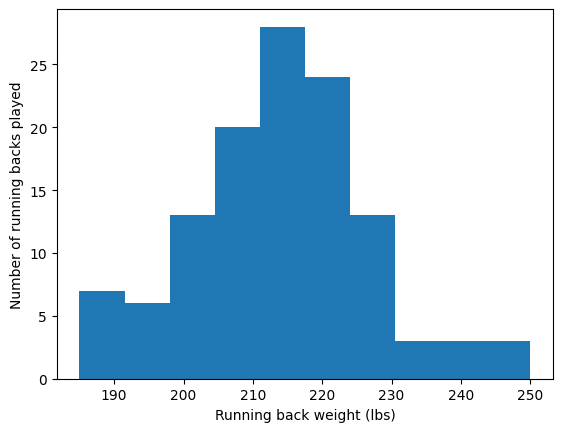
\includegraphics[width=\linewidth]{running-back-weight.png}
  \caption{Histogram of played running back weight}
\end{figure}

\begin{figure}[h]
  \centering
  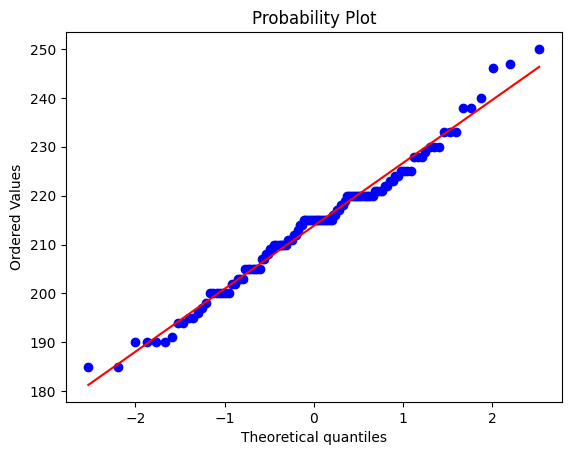
\includegraphics[width=\linewidth]{running-back-weight-qq.png}
  \caption{QQ plot of played running back weight}
\end{figure}

We binned running backs by weight into 5 bins to determine if running back
weight had an affect on the number of plays with at least one missed tackle.
Ultimately, it was inconclusive whether running back weight had a significant
impact on tackle performance. The dataset lacked a sufficient number of missed
tackle observations to meet our target number of at least 5 for each bin.

\begin{table}[H]
  \caption{Running back weight and play counts}
  \label{tab:freq}
  \begin{tabular}{lll}
    \toprule
    Weight category & Missed tackle & Tackle or assist (not missed) \\
    \midrule
    185 - 198 & 4 & 463 \\
    198 - 211 & 9 & 2007 \\
    211 - 224 & 17 & 2504 \\
    224 - 237 & 14 & 1078 \\
    237 - 250 & 2 & 596 \\
  \end{tabular}
\end{table}

\subsubsection{Increasing passing yards}

Examining the distance the quarterback passes the ball, we can see that
distribution of passes is strongly skewed right with 1st and 3rd quartiles of 0,9.
This indicates that most passes tend to be low with most falling between -5 and
10 as shown by the bar chart below
\begin{figure}[h]
  \centering
  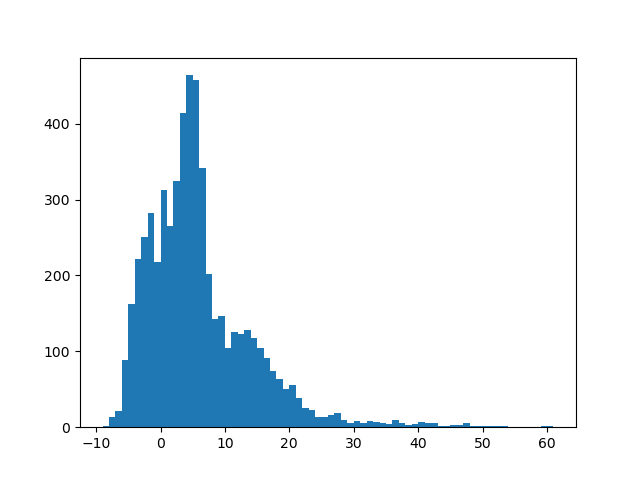
\includegraphics[width=\linewidth]{passlength}
  \caption{length of passes}
\end{figure}

Comparing the pass result with passing yards, we can see that the most play results
tend to be higher than the yards passed because players will try to move the
ball forward.
\begin{figure}[h]
  \centering
  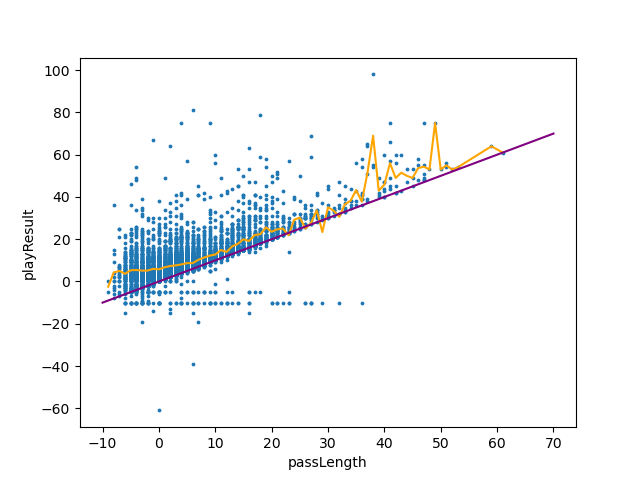
\includegraphics[width=\linewidth]{length_v_result}
  \caption{pass length vs result}
\end{figure}
It is also noticeable that several outliers fall below this line which can be
explained by penalty points of 5 or 10 or if the ball was intercepted by the
opposing team. There are also some outliers which are very far above the average
distance the player goes which indicates the carrier was able to dodge most of
the defenders.

Examining the difference between play result and pass length (figure
\ref{fig:pl}) as a proxy for the amount of distance an offensive player goes
before being tackled, we can see that in the range of approximately [-5,8], the
average distance before tackle decreases as the pass length increases probably
because at these distances, other team members can help prevent the ball carrier
from being tackled. The average distance covered changes by -0.76231569 yards
for each extra yard the pass covers. Note that this linear regression has score
of 0.027 which indicates the data is likely not linear.

We can also see that the play result seems to be the primary variable used by
the NFL to predict the expected score for a game(represented by the color of a
point) and that the prediction ``penalizes'' teams which have their ball
intercepted presumably because this indicates a lack of skill.
\begin{figure}[h]
  \centering
  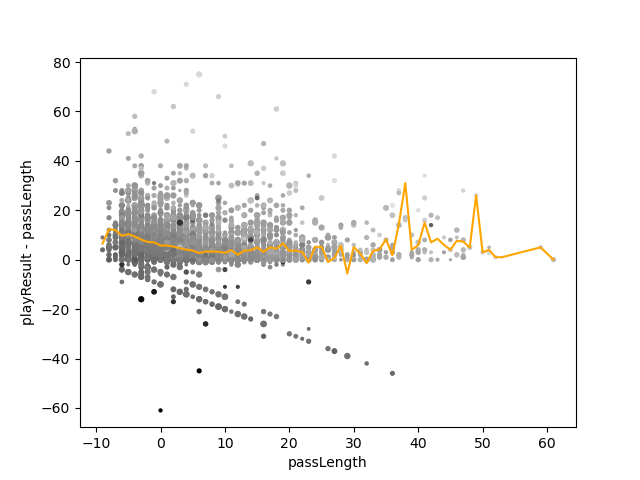
\includegraphics[width=\linewidth]{result-length}
  \caption{pass length vs distance before tackle}
  \Description{The color of dots represents the team's projected score after the play,
    the orange line is the average distance traveled after catching the ball}
  \label{fig:pl}
\end{figure}

\subsubsection{Choosing specific offensive formation types}

Examining the Plays data, we found six formation types played by offenses:
Empty, I-formation, Jumbo, Pistol, Shotgun, Singleback, and Wildcat. Overall,
Shotgun is the most popular formation type, followed by Singleback.

\begin{figure}[h]
  \centering
  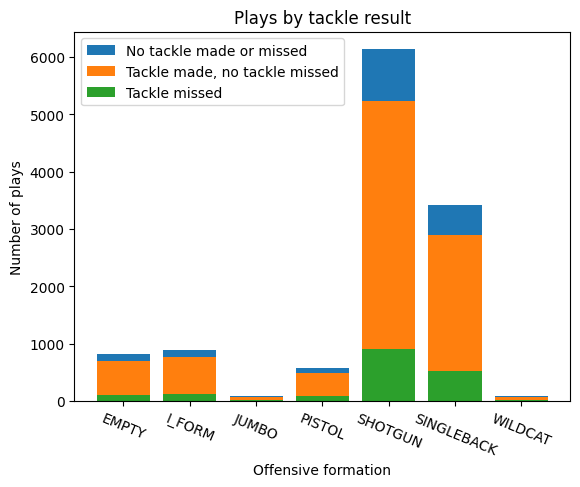
\includegraphics[width=\linewidth]{plays-by-tackle-result.png}
  \caption{Plays by tackle result, grouped by offensive formation}
\end{figure}

However, formation distributions change based on down and distance. One special
case is third and long situations (yards to go greater than 10, as a result of
penalties, quarterback sacks, or other negative yardage plays). For these plays,
picking up a large amount of yards is crucial to the offense maintaining
possession of the ball.

For third and long situations we found that the popularity of the Singleback
formation dropped considerably, and the popularity of the Empty formation rose
considerably, compared to the overall distribution. This supports a conclusion
that Empty formations are optimized for long passes down the field, which may
have a lower chance of success overall but are seen as necessary to convert a
third and long.

\begin{figure}[h]
  \centering
  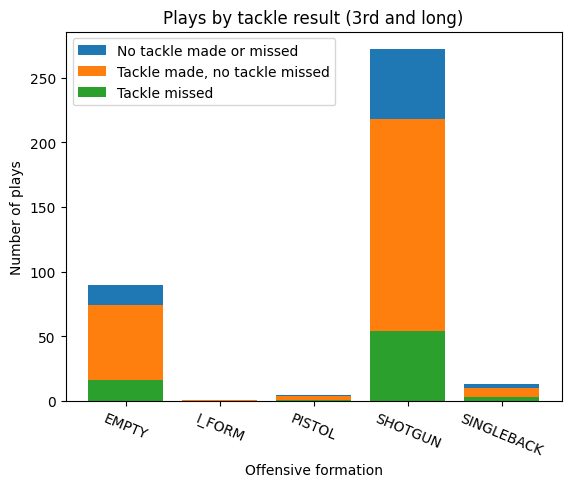
\includegraphics[width=\linewidth]{plays-by-tackle-result-third-and-long.png}
  \caption{Plays by tackle result in third and long situations, grouped by
  offensive formation}
\end{figure}

Missed tackles are very detrimental for a defense, as the majority of offensive
touchdown plays involved at least one.

\begin{figure}[h]
  \centering
  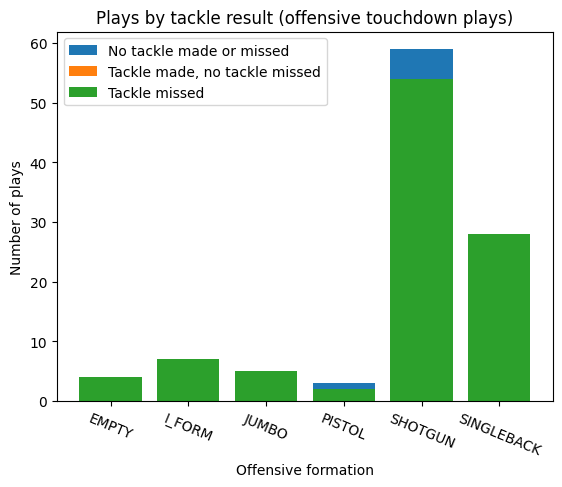
\includegraphics[width=\linewidth]
  {plays-by-tackle-result-offensive-touchfown-plays.png}
  \caption{Plays by tackle result resulting in an offensive touchdown, grouped
  by offensive formation}
\end{figure}

We performed a chi-squared test to determine if offensive formation had an
affect on the number of plays with at least one missed tackle. Ultimately, with
\textit{p} = 0.888, it was insufficient to disprove the null hypothesis and find
that the offensive formation had a significant impact on tackle performance. The
dataset lacked a sufficient number of missed tackle observations and was heavily
imbalanced toward certain offensive formations.

\subsection{Tackles as a predictor of victory}

To determine if the quantity of tackles themselves contributed to the
likelihood of winning a game, another na\"ive Bayesian classifier was
constructed based on the number of successful tackles performed by each team
during a game.

From the provided dataset of tackles, the number of successful tackles was
aggregated by game and team. This was then combined with whether or not the
team won the game in question. From there, the number of tackles made by a team
during one game was bucketed into three categories: "High" (over 61 made
tackles), "Average" (between 45 and 61 made tackles, inclusive), and "Low"
(under 45 made tackles). This information was then used as the attribute for a
Bayesian classifier to predict likelihood of victory based on the number of
successful tackles.

The resulting classifier had an accuracy of $60\%$ and an F1-score of
$0.6178628389154706$. Broadly, it categorized a "High" number of tackles as a
lost game, and an "Average" and "Low" number of tackles as a won game. Thus, it
does not appear as if the number of successful tackles has a significant impact
on the likelihood of victory. Additionally, when the model was slightly
modified to predict victory based on the number of missed tackles, the results
were comparable.

Again, however, the accuracy scores were likely affected by the low proportion
of missed to made tackles in the dataset. When the dataset was adjusted with
SMOTE, the accuracy was then about $57.8\%$, and the F1-score was
$0.5984794061302681$. Accuracy was therefore lower, but the general
implications with regard to the lack of applicability and predictive power of
the number of tackles remained the same.

\section{Discussion}

\subsection{Imbalance in missed tackle observations}

The missed tackle class in the tackles data, provided by the third-party vendor
Pro Football Focus as noted in the dataset description, contains a significantly
smaller number of missed tackle observations (2,090) than non-missed (15,336).
This imbalance made producing statistical significance when attempting to check
for a correlation between missed tackles and another variable, or training
classifiers to predict missed tackles, difficult. We were able to use Synthetic
Minority Over-sampling Technique (SMOTE) to partially mitigate this for
classifiers, but ideally we would have a much larger dataset to work with in
order to produce statistical significance in all our forms of analysis.

\subsection{Other sources of data}

This dataset is limited to only nine weeks of gameplay in the 2022 season, which
is a tiny sample of the decades of NFL gameplay data that exists. Websites such
as espn.com and footballdb.com have compiled extensive amounts of data on NFL
games, up to and including the current 2024 NFL season, and made it available to
the public. The catch? These websites haven't made it available as an easily
downloadable CSV file, requiring the use of a web scraper to collect it. They
also tend to lack the detailed play-by-play tackling and tracking data of this
NFL-provided dataset.

Nevertheless, many useful insights have been collected by these websites based
on the massive database of gameplay data they contain. A more extensive analysis
should also include data from these other sources when analyzing metrics such as
player weight and yards gained.

\subsection{Expanding project scope}

This project struggled to produce many useful results because of its narrow
focus on tackling which was believed to be well-suited to this dataset. Tackling
is just one of dozens of metrics which can be used to predict play and game
outcomes for NFL games. Perhaps the scope should've been expanded to embrace
other metrics for analysis more thoroughly.

Despite the narrow focus, some useful insights not related to tackling were
discovered throughout the analysis of this dataset. This included the weight
distribution of running backs, the length of passes, offensive formation type
preferences, and the yards to go distribution, across all the included NFL
plays.

\subsection{Utilization of tracking data}

We had considered using temporal data particularly the tracking data to see if
we can find any patterns over time. However, this was difficult due to the
lack of historical data, short period of the tracking data, and its
incompleteness i.e. only including a few frames around each notable event in the
game. This was deemed to be outside the scope of the project though possible of
interest for future projects.

\subsection{Reflection}

As with any form of data analysis, we aimed to find meaningful patterns and
trends that can illuminate bigger truths about our area of study without
unwarranted manipulation. Additionally, in order to conclude that these patterns
and trends are in fact meaningful, we must be able to disprove the null
hypothesis.

In essence, if we are mining the data for the effect of an example X variable,
the null hypothesis would state that there is no statistical difference in
tackle rate that can be attributed to X variable, and that any observed
difference is due to nothing more than chance. Thus, in order to disprove it,
the pattern would need to appear a sufficient amount of times within the dataset
to surpass the significance level (typically set at 5\%).

Notably, this is not the same as \textit{proving} the hypothesis. Rather, we
only had the ability to disprove that it does not hold. This is often the case
with real-world data, and we are still be able to present our findings with some
significance if that is the case.

In addition to these metrics, we evaluated our work based on the thoroughness of
our investigation and our consideration of all factors. Real-world data is
rarely straightforward, and contains many confounding variables that can all
have impacts on the observed results. Accordingly, we didn't make make finding
an “answer” our goal, but instead focused on exploring the data as best we can.

Even if we were unable to find conclusive or applicable implications for play strategies,
we value what information our work does provide, and look forward to the future work
that may result.

\section{Conclusion}

\subsection{Predicting tackle success}

We used three main methods of prediction of tackles' success:
clustering tackles by position, speed, etc and finding clusters of success or failure,
using classifiers and to predict whether a tackle will occur and if it succeeds,
and analyzing potential offensive and defensive strategies to see if they have an effect.

% \subsubsection{Exploratory analysis}
Most tackles occur fairly close to the starting line of a play (i.e. with 10 yards to go)
generally ahead of it. Additionally, fouls by either team can move the starting
point by 5 or 10 which can be identified as oddities in the data.

% \subsubsection{Grouping tackles}
Attempting to group tackles using k-means clustering, we were unable to find
any significant clusters of failure or success. We were able to determine that
tackles tend to be more densely clustered close to the center of the field and
players are likely to be going in the same directions when tackling and the ball
carrier tends to be going at higher speed. Players also tend to have lower speed
and acceleration at the moment of tackle regardless of success.

\subsubsection{Classifying tackles}

% TODO: Add conclusion (Isaac & Tim)

Initially, it appears as if player attributes have a fairly strong
correlation with their likelihood of being tackled. However, this is likely due
to the prevalance of made/successful tackles in the dataset, and therefore the
relative scarcity of missed tackles.

When the dataset is adjusted for this using SMOTE, the accuracy and F1-scores of
the models greatly decrease. As a result, we were not able to find a meaningful association
between player characteristics of height, weight, and position, and their likelihood
of being tackled.

\subsection{Offensive strategies}

We tested three offensive strategies for their usefulness:
the weight of running backs, increasing passing yards, and offensive formations.

\subsubsection{Optimizing the weight of running backs}

The weight of played running backs is roughly normally distributed, \textit{m} =
213.82 pounds, \textit{sd} = 12.75 pounds. Running backs aren't significantly
heaver than other offensive players. We were not able to find an association
between running back weight and missed tackles.

\subsubsection{Increasing passing yards}

With shorter passes, the distance players can go before being tackled is
decreasing possibly because they are more likely to get surrounded. This effect
is on average overshadowed by the extra yards gained by longer passes.
There is also very little data for long passes but there is some data to suggest
that long passes can lead to longer runs without being tackled.

\subsubsection{Choosing specific offensive formation types}

The dataset contains six offensive formation types, with Shotgun and
Singback being the most popular overall. Offensive formation preferences change
based on down and distance, suggesting that some formations work better
depending on what the offense's goals are. We were not able to find an
association between offensive formation and missed tackles.

\subsection{Tackles as a predictor of victory}

As previously noted, the provided dataset is unfortunately limited in terms of the representation of
missed tackles. Many more made tackles are available in the data, and thus predictive classifiers are
skewed towards them.

Even so, the number of made (or missed) tackles does not have strong predictive ability with regards to
a team's victory, whether or not the dataset was adjusted with SMOTE. We were not able to find an
association between number of tackles and winning games.

\bibliographystyle{ACM-Reference-Format}
\bibliography{sources}
\nocite{*}

\section{Appendix}

\subsection{Honor Code}

On my honor as a University of Colorado Boulder student I have neither given nor
received unauthorized assistance.

\subsection{Individual contributions}

\begin{itemize}
  \item Isaac Kou
  \begin{itemize}
    \item Classifying tackles: Na\"ive Bayesian
    \item Classifying tackles: Decision tree
    \item Tackles as a predictor of victory: Na\"ive Bayesian
    \item Classifying tackles \& Tackles as a predictor: SMOTE re-analysis
  \end{itemize}
  \item Sean Shi
  \begin{itemize}
    \item Exploratory analysis
    \item Grouping tackles: k-means analysis of football speed and acceleration
    \item Offensive strategy: Increasing passing yards
  \end{itemize}
  \item Timur Tripp
  \begin{itemize}
    \item Grouping tackles: k-means analysis of football position
    \item Offensive strategy: Optimizing the weight of running backs
    \item Offensive strategy: Choosing specific offensive formation types
    \item Classifying tackles: Random forest
  \end{itemize}
\end{itemize}
\end{document}
\endinput
